\chapter{Strumentazione}
\label{chap:tools}

\section{Piattaforma di sviluppo}
\label{sec:platform}
La workstation usata per lo sviluppo del software è un server Linux con 2 schede video NVIDIA Titan X ed è collegata alla rete con IP pubblico all'indirizzo solaris.micc.unifi.it ed accedibile con utente mtintori. 
La modalità di lavoro perseguita è remota utilizzando remote desktop da PC Windows e PC Mac in seguito.
L'IDE utilizzato per lo sviluppo è Pycharm con versione di Python 3.6.

\section{Miniconda}
Miniconda è un gestore di pacchetti ed environment-manager. E' una versione di installazione minimale di Anaconda, comprende l'interprete Python e permette di utilizzare un'IDE alternativo a Spider, usato con Anaconda, inoltre non vengono installati gli oltre 250 pacchetti che sono compresi nell'installazione di Anaconda lasciando la libertà allo sviluppatore su quali pacchetti installare.
\label{sec:miniconda}
\subsection*{Ambienti Miniconda}
Utilizzeremo il termine Conda, istruzione fondamentale Miniconda, per riferirsi al sunnominato manager.
Per la realizzazione del Codec si è resa necessaria la creazione di due ambienti Conda: è stata effettuata una simile scelta per possibilità di debug anche in assenza di rete su una workstation personale che non possiede una GPU. 
\begin{itemize}
\item \emph{tf\_cpu} : ambiente più lento, ma utilizzabile anche da una workstation non avente GPU
\item \emph{tf\_gpu} : ambiente più veloce, ma utilizzabile solo da una workstation con una GPU con ampia memoria adatta al training di reti neurali
\end{itemize}
\section{Schema del sistema}
\begin{figure}
   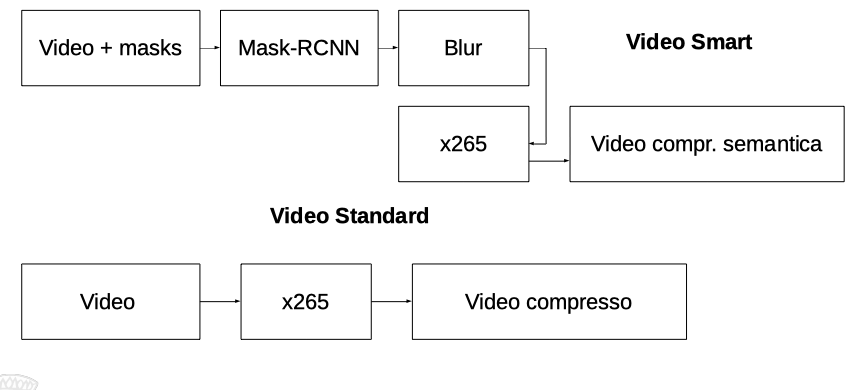
\includegraphics[width=\linewidth]{images/schema.png}
   \caption{Sistema}
   \label{fig:c}
\end{figure}
\section{CODEC di partenza}
\label{sec:codec_base}
%Descrivere il codec
La scelta del codec da utilizzare era contesa tra gli standard candidabili \textbf{H.264}, \textbf{H.265}, mentre gli altri due standard ottimali \textbf{VP9} e \textbf{AV1} non sono stati volontariamente presi in considerazione come assunto iniziale, nonostante le performance del secondo qualche volta superiore a \textbf{H.265} implementato dall'encoder \textbf{x265}.\textsuperscript{\ref{fig:c}} (si noti che \textbf{VP9} invece è visibilmente inferiore agli altri,come si nota pur dalle info \textbf{libvpx}\textsuperscript{\cite{libvpx}} che lo implementa).
\begin{figure}
   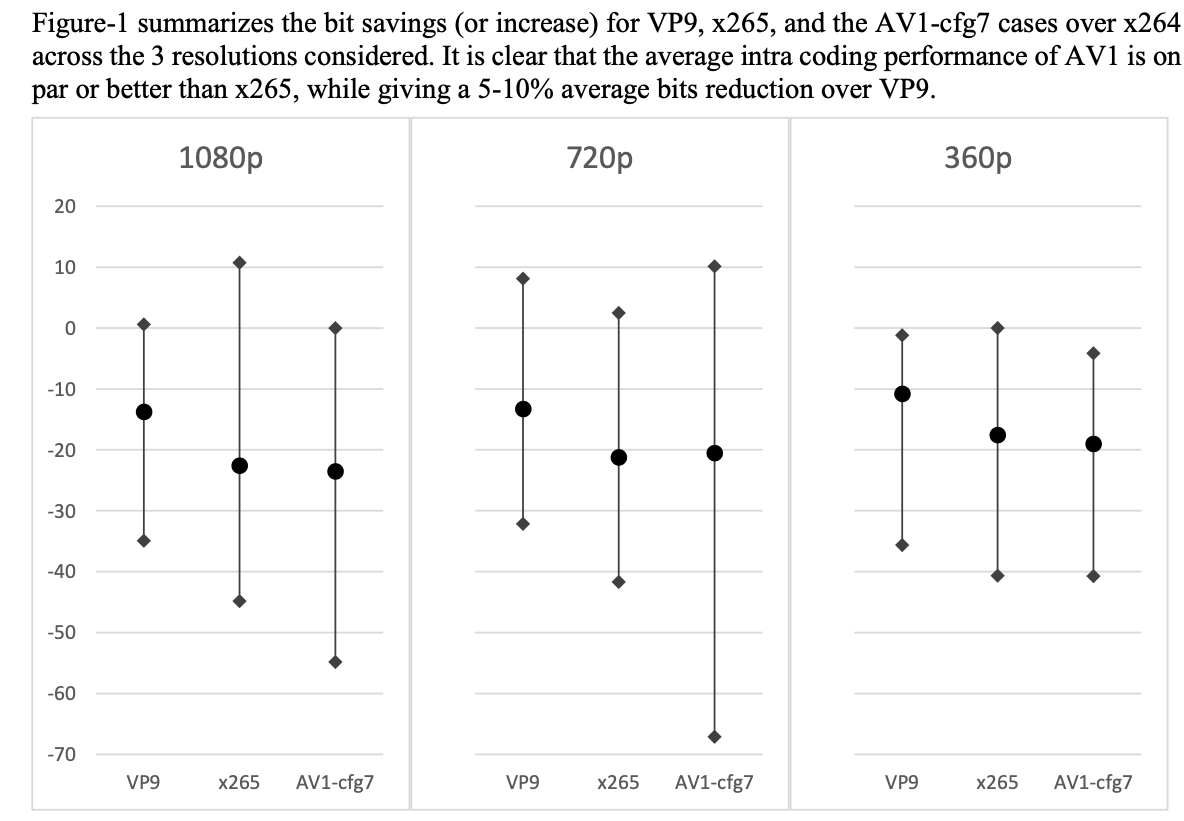
\includegraphics[width=\linewidth]{images/x265vsAv1.png}
   \caption{Risparmio in bits (segni: - risparmio, + incremento)}
   \label{fig:c}
\end{figure}
\\Sappiamo anche che \textbf{x264} implementa lo standard precedente; è quindi sicuramente più scarso. Lo standard dalla quale siamo partiti per una codifica efficiente è allora \textbf{H.265} usando \textbf{hevc\_nvenc} \textsuperscript{\ref{sec:nvenc}}, ed abbiamo optato per una codifica progressiva frame per frame. Il nostro encoder prevede una quantizzazione "doppia", poiché prima di scrivere ogni frame vengono selezionate le regioni non interessanti e ne vengono tagliate fuori le HF\footnote{Alte frequenze}; ciò verrà spiegato in seguito. Quello che invece fa il Codec di partenza che abbiamo scelto è una quantizzazione secondo lo standard, che viene effettuata manovrando il parametro \emph{QP} cui valore rappresenta la sua intensità, ovvero quanta informazione (sempre HF) viene scartata.
\subsection*{CRF}
Il Costant Rate Factor\textsuperscript{\cite{CRF_vs_QP}}  è un fattore che influenza la quantizzazione in modo più sofisticato del parametro a basso livello \emph{QP} previsto dallo standard H.265. Più alto il CRF, più i campioni (pixel o blocchi di pixel) vengono quantizzati in maniera maggiore; questo valore resta fisso per l'intera codifica del video scelto, mentre il valore del parametro \emph{QP} varia a seconda di quanto si debba quantizzare in ogni frame per mantenere una qualità costante.
Nel nostro caso, utilizzando \textbf{nvenc} non sarà presente il parametro \emph{crf} ma si deve utilizzare il parametro equivalente \emph{cq} di questa libreria a cui sarà dato un valore che garantirà una compressione visivamente lossless, ovvero con perdita di qualità trascurabile all'occhio umano; essenzialmente questo valore per \textbf{h264\_nvenc} è circa 19 per cui, preso atto che il valore di default di \textbf{x264} è 23 e corrisponde a circa 28 di \textbf{x265}, non sbaglieremo nel dire che 19 è sicuramente visually lossless anche per \textbf{hevc\_nvenc}.
\section{FFMPEG}
\label{sec:coding_library}
%Descrivere il codec
Utilizzando la libreria \textbf{FFMPEG} è stato possibile scegliere diversi parametri oltre al Codec \textbf{hecv\_nvenc}. 
Le modalità tipiche di codifica sono 3: \footnote{vedi rate control modes: https://trac.ffmpeg.org/wiki/Encode/H.265} 
\begin{enumerate}
\item bitrate scelto in 1 passo (sconsigliato)
\item bitrate scelto in 2 passi
\item CRF (fattore di qualità costante)
\end{enumerate}
Dal momento che non è nostro interesse il raggiungimento di una dimensione file particolare, la scelta è caduta sulla terza opzione, che è stata spiegata nella sottosezione precedente.
Gli altri parametri che abbiamo utilizzato per la codifica sono i seguenti:
\begin{itemize}
\item \textbf{-cq}: fattore di qualità che mantiene la suddetta costante in ogni frame manovrando il parametro che definisce la quantizzazione \emph{QP}
\item \textbf{-qmin} : fattore minimo di qualità che \textbf{cq} può assumere
\item \textbf{-qmax} : fattore massimo di qualità che \textbf{cq} può assumere
\item \textbf{-b:v} : posto a 0 per causa di un bug nella libreria, che se non venisse settato inibisce il funzionamento di cq
\item \textbf{-rc} : rate control, sovrascrive la velocità di compressione ("preset",più basso il preset più alta la qualità) e deve essere settato insieme a \textbf{\emph{-b:v}} per una qualità costante
\item \textbf{-r} : frame rate, ovvero quanti frame vengono campionati nell'unità di tempo
\end{itemize}
%Descrivere l'ambiente in cui opererà il software, includendo piattaforme hardware, altri sistemi operativi con relativa versione, altre componenti software che utilizza questo prodotto

\section{Mask-RCNN}
\label{sec:Mask-RCNN_desc}
Mask-RCNN è un'implementazione di una rete neurale Faster-RCNN da parte del framework tensorflow di Google. Si differenzia dalle Faster-RCNN per l'introduzione del RoI Align, più preciso rispetto al RoI Pooling precedente. Facciamo un piccolo riepilogo per maggiore chiarezza.
\subsection*{Riepilogo - Dalle CNN alle Faster-RCNN}
Le reti neurali convoluzionali \textbf{(CNN)} sono state introdotte nel campo dell' IA per vari scopi e più precisamente nella computer vision sono utili per il riconoscimento di qualsiasi entità o pattern all'interno di un immagine. Le potenzialità e i limiti sono elencati di seguito:
\begin{enumerate}
\item Usano una funzione softmax per classificazione multi-classe e sigmoid per classificazione binaria
\item Usata per image classification e object detection
\item Rileva solo un oggetto alla volta senza sovrapposizioni
\end{enumerate}
Successivamente si sono affermate le CNN basate su regioni \textbf{(RCNN)}, che forniscono il miglioramento di riconoscere più oggetti diversi nella stessa immagine e identificarli all'interno di un rettangolo. Questo è possibile con il seguente procedimento:
\begin{enumerate}
\item Generazione di regioni propositive con R-CNN per mezzo dell'algoritmo \emph{Selective Search} unito con \emph{Exhaustive Search}
\item Fusione di regioni propositive simili e \emph{Feature extraction} con CNN per ogni regione propositiva
\item Algoritmo \emph{Support vector machine} per la feature estratta per la verifica dell'effettiva presenza dell'oggetto 
\item Algoritmo \emph{Non-Max suppression} per lo scarto di regioni con basso punteggio in \emph{Intersection over Union}.
\end{enumerate}
Per ottenere un altro significativo miglioramento siamo arrivati alle reti \textbf{Fast-RCNN}, che offrono i seguenti vantaggi:
\begin{enumerate}
\item Unica rete neurale (deep ConvNet) che sostituisce quelle migliaia di R-CNN sulle singole regioni
\item Unico modello per la feature extraction, la classificazione e le bounding boxes
\item Introduzione delle Region of Interest (RoI) e del RoI Pooling
\end{enumerate}
Infine, si è voluto perfezionare l'arte del riconoscimento e identificazione delle forme di ogni entità con le reti \textbf{Faster-RCNN}, che permettono di:
\begin{enumerate}
\item 3-D object detection
\item Part-based detection
\item Instance segmentation
\item Image captioning
\end{enumerate}



